\documentclass[conference]{IEEEtran}
\IEEEoverridecommandlockouts
\usepackage{cite}
\usepackage{amsmath,amssymb}
\usepackage{graphicx}
\usepackage{booktabs}
\usepackage{xcolor}
\usepackage{url}
\usepackage{listings}
\graphicspath{{../../project_artifacts/diagrams/}{../../project_artifacts/screenshots/}}
\lstset{basicstyle=\ttfamily\scriptsize, frame=single, columns=fullflexible, keywordstyle=\bfseries,
        language=Verilog, breaklines=true, xleftmargin=2pt, xrightmargin=2pt}

\begin{document}

\title{Design and Implementation of a 4$\times$4 Systolic Array Accelerator for Matrix Multiplication Using Verilog HDL}

\author{\IEEEauthorblockN{Yash Dhankhar}
\IEEEauthorblockA{\textit{B.Tech Computer Science \& Artificial Intelligence} \\
\textit{Newton School of Technology, Rishihood University}\\
India \\
yash.2024@nst.rishihood.edu.in}}

\maketitle

\begin{abstract}
Matrix multiplication dominates the workload of neural-network inference and many signal-processing algorithms. This paper presents the design, verification and FPGA implementation of a 4$\times$4 output-stationary systolic array that computes $C = A \times B$ on signed Q8.8 fixed-point operands. Sixteen processing elements, each with a two-stage pipelined multiply-accumulate (MAC) unit and a 34-bit overflow-free accumulator, are connected so that operands of $A$ flow horizontally and operands of $B$ flow vertically. Diagonally skewed input buffers, a six-state controller, an output register and a host interface complete the accelerator. Four self-checking testbenches compare every result element against independently computed references, and mutation testing confirms that the testbenches detect injected faults. In simulation the accelerator completes a 4$\times$4 product in 14 clock cycles, versus 64 cycles for a single-MAC sequential design. After placement and routing on a Lattice ECP5-25F FPGA it reaches a median 122.0\,MHz, giving 114.7\,ns per product, 6.7$\times$ faster than the sequential design, at a cost of 16 hardware multipliers instead of one.
\end{abstract}

\begin{IEEEkeywords}
systolic array, matrix multiplication, multiply-accumulate, fixed-point arithmetic, Verilog HDL, FPGA, hardware accelerator
\end{IEEEkeywords}

\section{Introduction}
The product $C = A B$ of two $N\times N$ matrices is defined element by element as
\begin{equation}
C_{ij} = \sum_{k=0}^{N-1} A_{ik} B_{kj}, \qquad 0 \le i,j < N,
\label{eq:mm}
\end{equation}
which requires $N^3$ multiply-accumulate (MAC) operations. A conventional processor with one MAC unit therefore needs at least $N^3$ cycles. Every term in (\ref{eq:mm}) is independent of the others except through the final sum, so the computation is highly parallel. Systolic arrays, introduced by Kung and Leiserson \cite{kung1979}, exploit this with a regular grid of simple processing elements (PEs). Data are fetched once from memory and then pumped rhythmically from neighbour to neighbour, so each operand is reused by many PEs without further memory traffic \cite{kung1982}. The same principle underlies modern deep-learning accelerators such as Google's Tensor Processing Unit \cite{jouppi2017}.

This project designs a small but complete systolic accelerator in synthesizable Verilog \cite{ieee1364}. Its contributions are:
(i) a parameterized 4$\times$4 output-stationary array with signed Q8.8 arithmetic and an accumulator width that provably cannot overflow;
(ii) a complete datapath and control around the array (skewed input buffers, controller, output register, host interface);
(iii) self-checking verification, including mutation testing of the testbench itself; and
(iv) measured latency, throughput, and post-place-and-route FPGA results compared against a sequential baseline that has the same interface.

\section{Literature Review}
Kung and Leiserson \cite{kung1979} described systolic arrays for matrix operations and showed how hexagonal and orthogonal arrays can perform matrix multiplication with nearest-neighbour communication only. Kung \cite{kung1982} later argued that systolic designs suit VLSI because they balance computation with I/O bandwidth, use simple and regular cells, and avoid long global wires. S.~Y.~Kung \cite{kung1985} generalized these ideas into the wider class of VLSI array processors and formalized how algorithms are mapped onto them.

The approach became central to machine-learning hardware. The first-generation TPU \cite{jouppi2017} uses a 256$\times$256 systolic array of 8-bit MACs, a weight-stationary design in which weights are preloaded and activations flow through the array. Eyeriss \cite{chen2017} studied how the choice of which operand stays inside a PE (the \emph{dataflow}) affects energy, and proposed a row-stationary dataflow. Sze \emph{et al.} \cite{sze2017} survey these dataflows: weight-stationary, output-stationary and row-stationary. Gemmini \cite{genc2021} is an open-source generator of systolic accelerators that supports both output- and weight-stationary dataflows, and SCALE-Sim \cite{samajdar2018} models the cycle behaviour of systolic arrays for CNN workloads.

This project uses the \emph{output-stationary} dataflow. Each PE keeps one element of $C$ in its accumulator while $A$ and $B$ stream past. This dataflow needs no partial-sum movement between PEs and suits a small array whose results are read out after every job.

\section{Existing System and Limitations}
The reference point is a conventional sequential datapath. It has one multiplier and one adder, three nested loop counters $(i,j,k)$, and operand memories. For this work it was implemented as \texttt{sequential\_matmul.v}, with exactly the same host interface and arithmetic as the accelerator. Its limitations are:
\begin{itemize}
\item \textbf{Serial execution.} The $N^3=64$ MACs run one per cycle. The measured latency is 64 cycles and the sustained period is 65 cycles per product.
\item \textbf{No operand reuse.} Each $A_{ik}$ is read $N$ times and each $B_{kj}$ is read $N$ times from memory.
\item \textbf{Memory on the critical path.} The operand read, multiplier and adder are in one combinational path. The post-route clock is 83.2\,MHz (median) on ECP5.
\end{itemize}

\section{Proposed Solution}
The proposed accelerator replaces the single MAC with an $N\times N$ grid of MAC-based PEs (here $N=4$). The rows of $A$ enter from the left edge and the columns of $B$ from the top edge. Each input stream is delayed so that the operands of every term in (\ref{eq:mm}) meet in the correct PE at the same time. All 16 PEs then compute in parallel, each accumulating its own $C_{ij}$. The design was developed bottom-up: the PE was verified alone, then the array, then the complete system. Each step was checked against references computed independently in the testbench.

\section{System Architecture}
Fig.~\ref{fig:sys} shows the top-level organization. The host writes $A$ and $B$ element by element through \texttt{matrix\_interface}, which routes each write to the right buffer and ignores writes while the accelerator is busy. A \texttt{start} pulse makes \texttt{systolic\_controller} clear the array, stream the buffers into it, wait for the pipeline to drain, and capture all accumulators in \texttt{output\_register}. It then raises \texttt{done}. The host reads each $C_{ij}$ by address, either at full precision (\texttt{rd\_raw}) or rounded and saturated to Q8.8 (\texttt{rd\_q88}, with overflow flag \texttt{rd\_ovf}).

\begin{figure}[t]
\centering
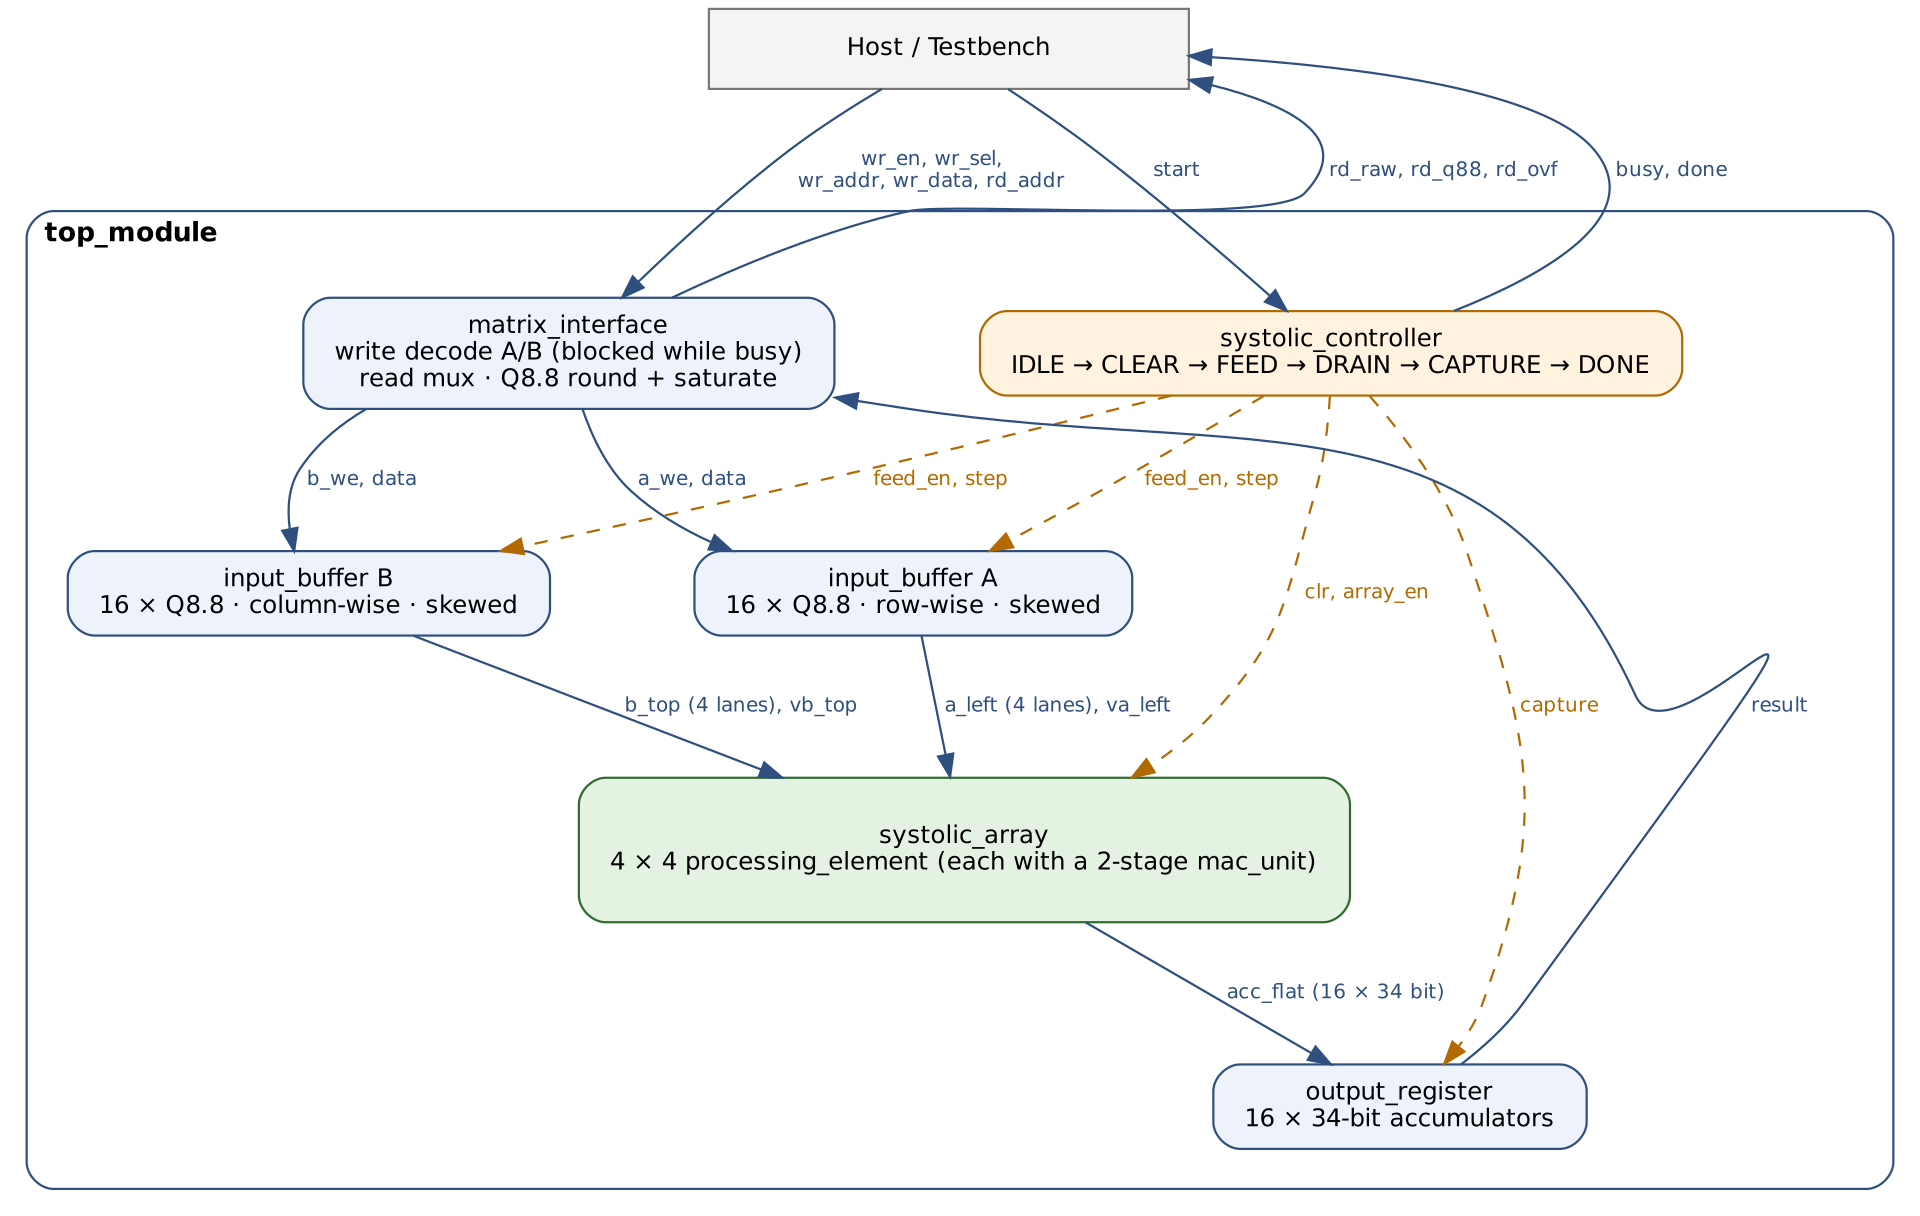
\includegraphics[width=\columnwidth]{system_architecture.png}
\caption{Top-level architecture of the accelerator (\texttt{top\_module}). Dashed lines are control signals from the controller.}
\label{fig:sys}
\end{figure}

\section{Hardware Design}
\subsection{Fixed-point number format}
Operands use signed Q8.8: a 16-bit two's-complement integer $x$ represents $x/2^8$, giving the range $[-128,\,127.996]$ in steps of $1/256$. The product of two Q8.8 numbers is Q16.16 (32 bits). The largest product magnitude is $(-2^{15})^2 = 2^{30}$, so a sum of $N$ products has magnitude at most $N\cdot 2^{30}$. The accumulator width is therefore chosen as
\begin{equation}
W_{acc} = 2W + \lceil \log_2 N \rceil = 2(16) + 2 = 34 \text{ bits},
\label{eq:accw}
\end{equation}
which holds $4\cdot2^{30} = 2^{32}$ with a sign bit to spare. No input can overflow the accumulator. The Q8.8 output is obtained by rounding to nearest and saturating:
\begin{equation}
y = \mathrm{sat}_{16}\!\left( \left\lfloor (acc + 2^{7}) / 2^{8} \right\rfloor \right).
\end{equation}

\subsection{Input buffers}
Each \texttt{input\_buffer} stores 16 words (address $r\cdot N + c$) and drives $N$ output lanes. The controller supplies a step counter $s = 0,\dots,2N-2$. At step $s$, lane $l$ outputs element $k = s-l$ if $0 \le k < N$, and otherwise a zero with its valid bit cleared. The A buffer is read row-wise (lane $l$ carries $A_{lk}$). The B buffer is read column-wise (lane $l$ carries $B_{kl}$). This produces the diagonal skew in Fig.~\ref{fig:grid}. The outputs are registered.

\subsection{Controller}
The controller (Fig.~\ref{fig:fsm}) is a Moore FSM with states IDLE, CLEAR, FEED, DRAIN, CAPTURE and DONE. FEED lasts $2N-1$ cycles, during which the step counter drives the buffers. DRAIN lasts $N+1$ cycles: one for the buffer register, $N-1$ for the last operands to hop to PE$(N-1,N-1)$, and one for the MAC pipeline. The total start-to-done latency is
\begin{equation}
L = 1 + (2N-1) + (N+1) + 1 = 3N + 2 = 14 \text{ cycles}.
\label{eq:lat}
\end{equation}
\texttt{done} stays high until the next \texttt{start}, so the host can poll it reliably.

\begin{figure}[t]
\centering
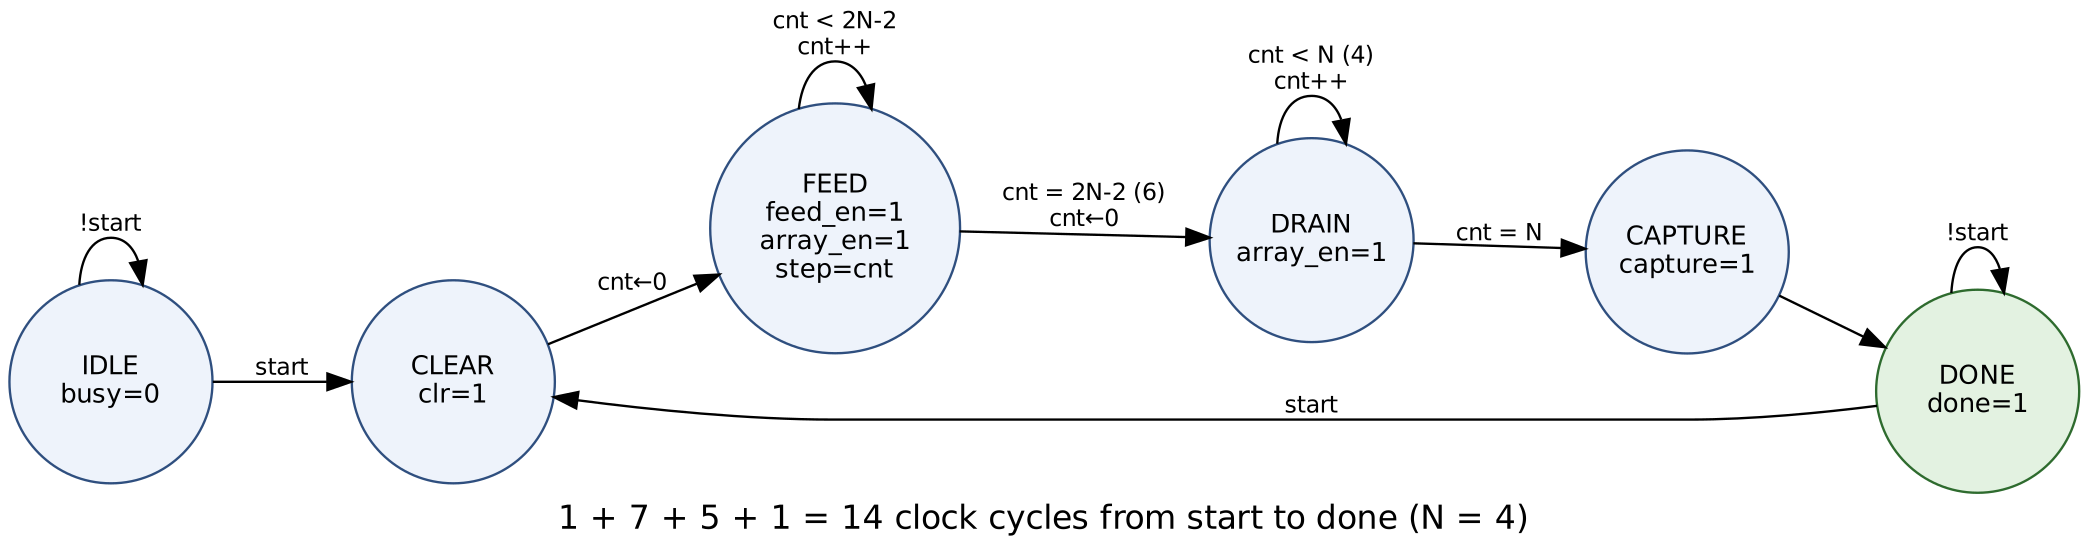
\includegraphics[width=\columnwidth]{controller_fsm.png}
\caption{Controller state machine (\texttt{systolic\_controller.v}).}
\label{fig:fsm}
\end{figure}

\section{Processing Element Design}
Each PE (Fig.~\ref{fig:pe}) contains a MAC unit and four forwarding registers: \texttt{a\_out}, \texttt{b\_out} and their valid bits. On every enabled clock, the PE passes $a$ to its right neighbour and $b$ to the neighbour below. The MAC accumulates only when the global enable and both valid bits are 1. Synchronous \texttt{rst} and \texttt{clr} reset the accumulator and the forwarding registers, so consecutive jobs cannot leak partial sums into each other. The global \texttt{en} input freezes the PE, which allows a whole-array stall.

\begin{figure}[t]
\centering
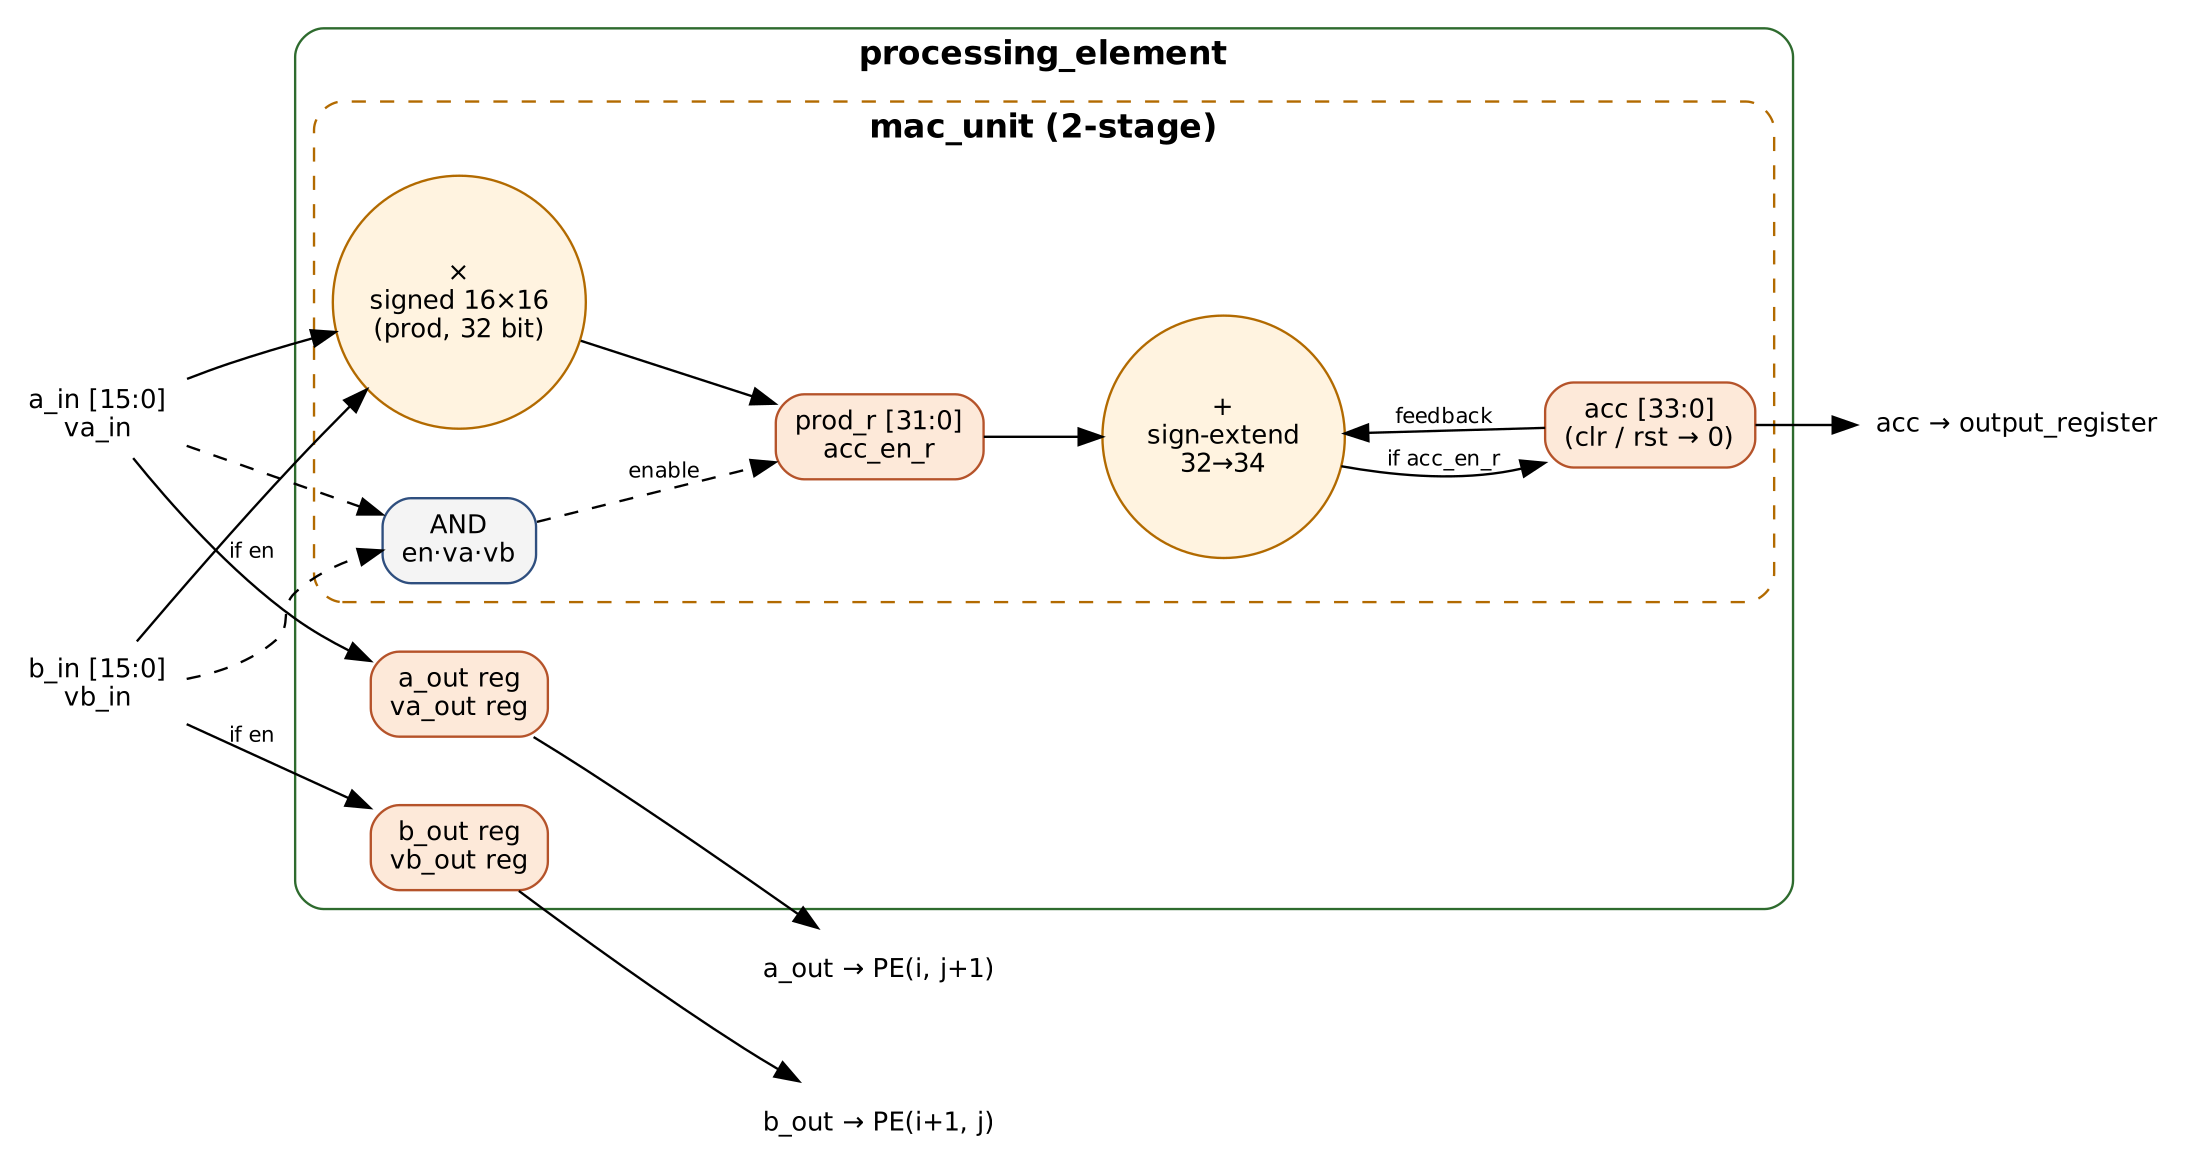
\includegraphics[width=\columnwidth]{processing_element_mac.png}
\caption{Processing element with its two-stage MAC unit.}
\label{fig:pe}
\end{figure}

\section{MAC Architecture}
The MAC unit has two pipeline stages:
\begin{align}
\text{stage 1:}\quad & p_r \leftarrow a \cdot b,\qquad e_r \leftarrow en \\
\text{stage 2:}\quad & acc \leftarrow acc + \mathrm{sext}_{34}(p_r)\ \text{ if } e_r = 1.
\end{align}
Both operands are declared \texttt{signed}, so the multiplier performs two's-complement multiplication. The 32-bit product is sign-extended to 34 bits before accumulation. A first version performed both stages in one cycle. Its post-route critical path ran from a forwarding register through the hard multiplier into the 34-bit adder (Section~\ref{sec:perf}), and the product register was added to break that path.

\section{Systolic Data Movement}
Fig.~\ref{fig:grid} shows the 4$\times$4 grid. Lane $i$ of the A buffer feeds PE$(i,0)$, and lane $j$ of the B buffer feeds PE$(0,j)$. Because of the skew, $A_{ik}$ leaves the buffer at step $k+i$ and then needs $j$ hops to reach column $j$. Likewise, $B_{kj}$ leaves at step $k+j$ and needs $i$ hops to reach row $i$. Both therefore arrive at PE$(i,j)$ at the same relative time
\begin{equation}
t_{ijk} = k + i + j,
\label{eq:arr}
\end{equation}
which is exactly when they must be multiplied for term $k$ of $C_{ij}$. Each operand is fetched from its buffer only once and reused by $N$ PEs as it travels.

\begin{figure*}[t]
\centering
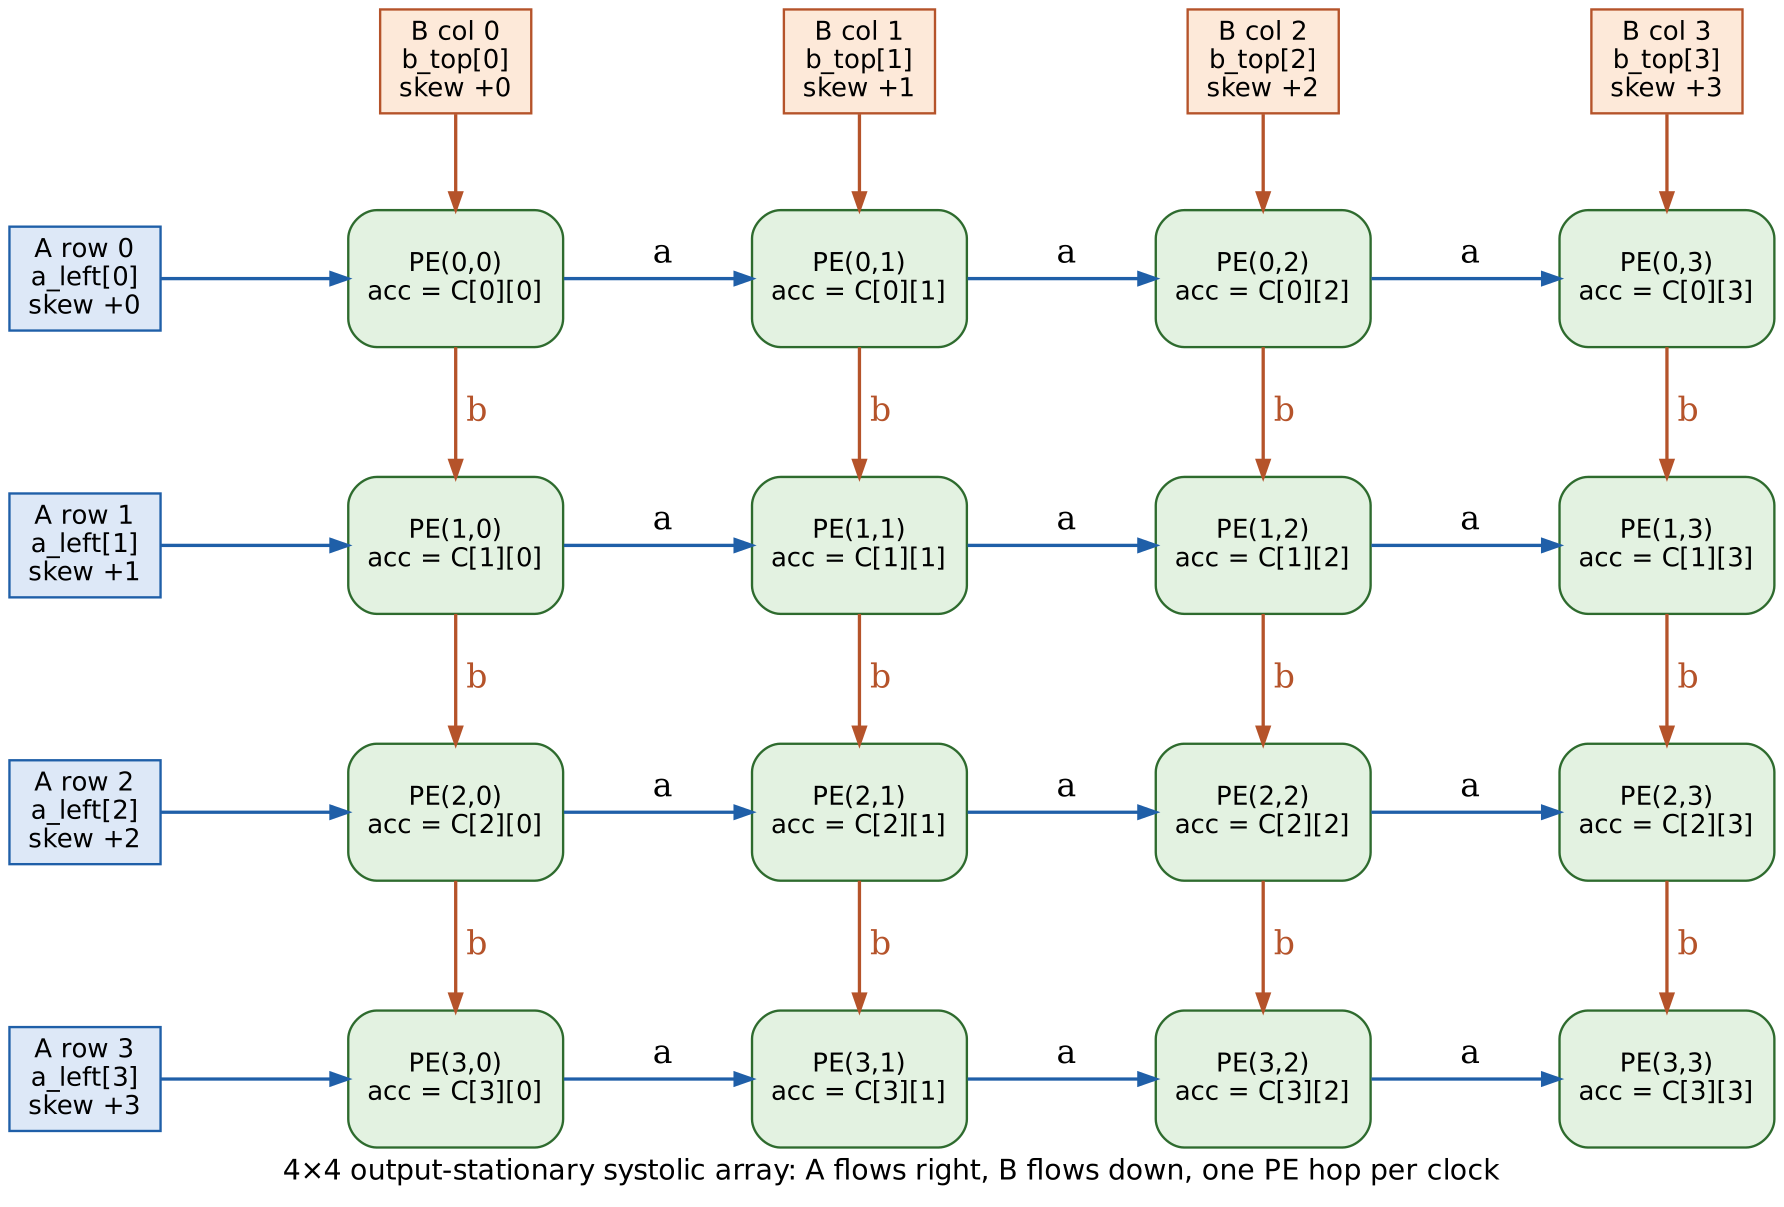
\includegraphics[width=0.78\textwidth]{pe_array_4x4.png}
\caption{The implemented 4$\times$4 output-stationary array. A moves right and B moves down, one PE per clock. Lane $i$ (or $j$) is delayed by $i$ (or $j$) cycles.}
\label{fig:grid}
\end{figure*}

\section{Verilog Implementation}
The design consists of eight synthesizable Verilog-2005 modules (Table~\ref{tab:mods}) plus the baseline. The array is built with nested \texttt{generate} loops. All buses between modules are flattened vectors, so the code stays within Verilog-2001/2005 and is accepted by both Icarus Verilog and Yosys. The key MAC code is:
\begin{lstlisting}
assign prod = a * b;            // signed 16x16
always @(posedge clk)
  if (rst || clr) begin
    prod_r <= 0; acc_en_r <= 0; acc <= 0;
  end else begin
    prod_r <= prod; acc_en_r <= en;
    if (acc_en_r)
      acc <= acc + {{(ACC_W-2*DW){prod_r[2*DW-1]}}, prod_r};
  end
\end{lstlisting}
All modules are parameterized by $N$, the data width and the accumulator width. The verification reported here covers $N = 4$.

\begin{table}[t]
\caption{RTL Modules}
\label{tab:mods}
\centering\footnotesize
\begin{tabular}{@{}ll@{}}
\toprule
Module & Function \\ \midrule
\texttt{mac\_unit} & 2-stage signed MAC, 34-bit accumulator \\
\texttt{processing\_element} & MAC + A/B forwarding with valid bits \\
\texttt{systolic\_array} & 4$\times$4 PE grid (\texttt{generate}) \\
\texttt{input\_buffer} & matrix storage, skewed lanes \\
\texttt{output\_register} & captures 16 accumulators \\
\texttt{systolic\_controller} & 6-state FSM, \texttt{busy}/\texttt{done} \\
\texttt{matrix\_interface} & host write/read, Q8.8 round+saturate \\
\texttt{top\_module} & integration \\
\texttt{sequential\_matmul} & single-MAC baseline \\ \bottomrule
\end{tabular}
\end{table}

\begin{figure*}[!t]
\centering
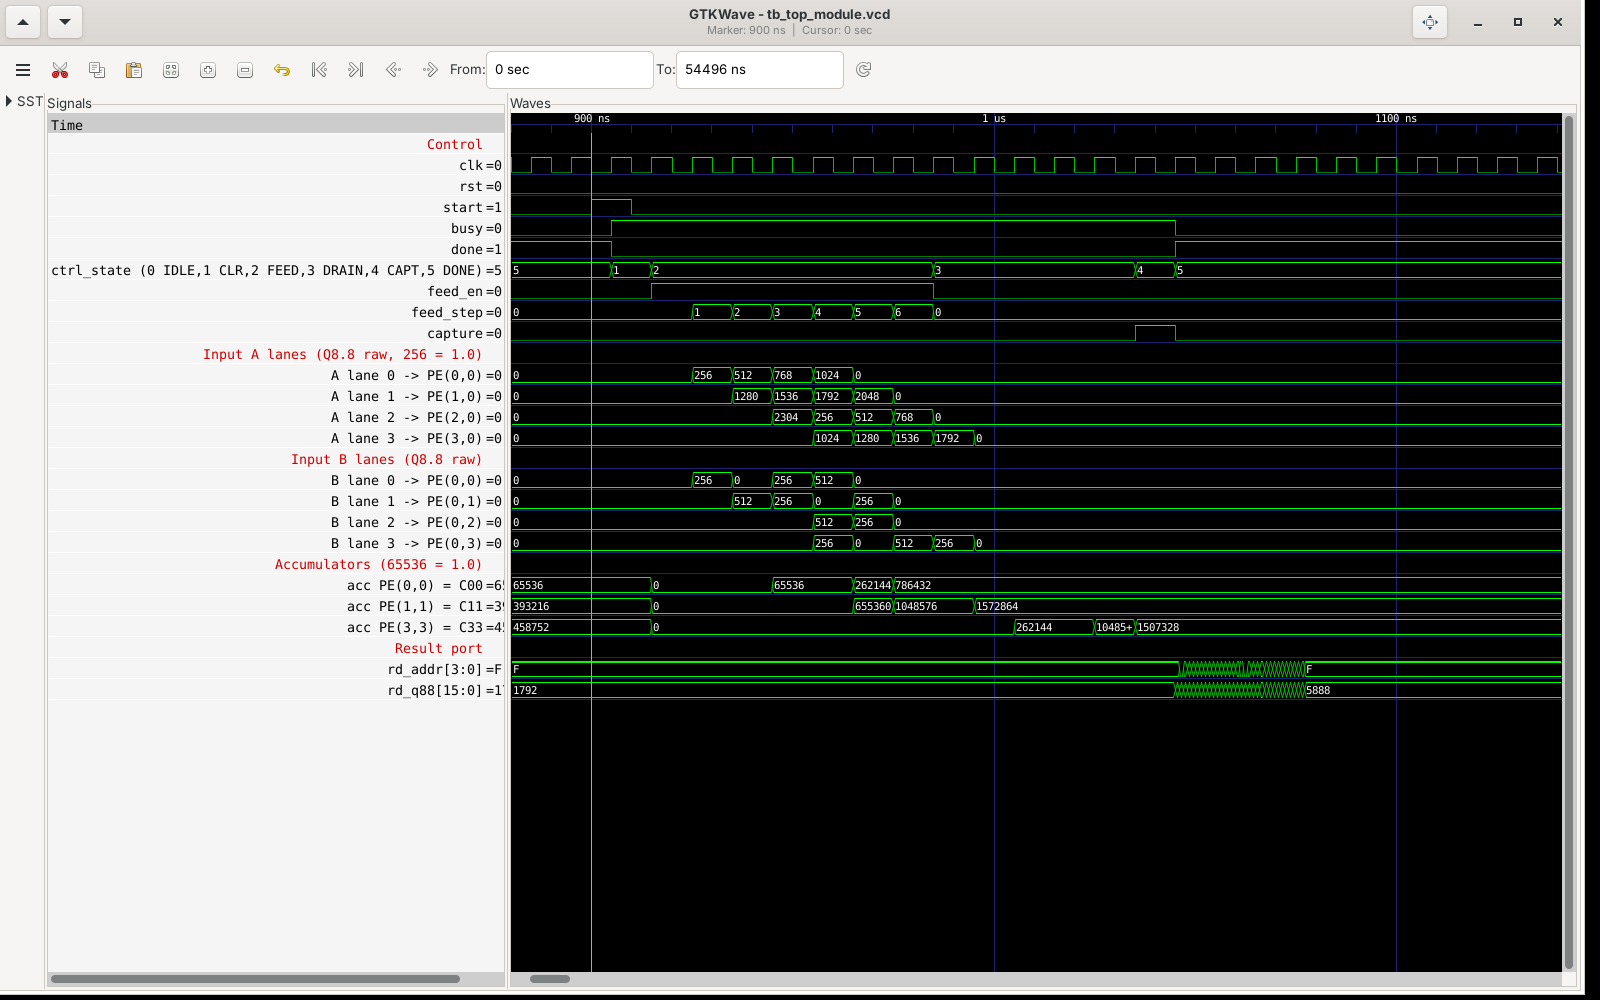
\includegraphics[width=0.80\textwidth]{03_full_waveform.png}\\[2pt]
{\footnotesize (a) Control signals, skewed A and B input lanes, accumulators and result port.}\\[6pt]
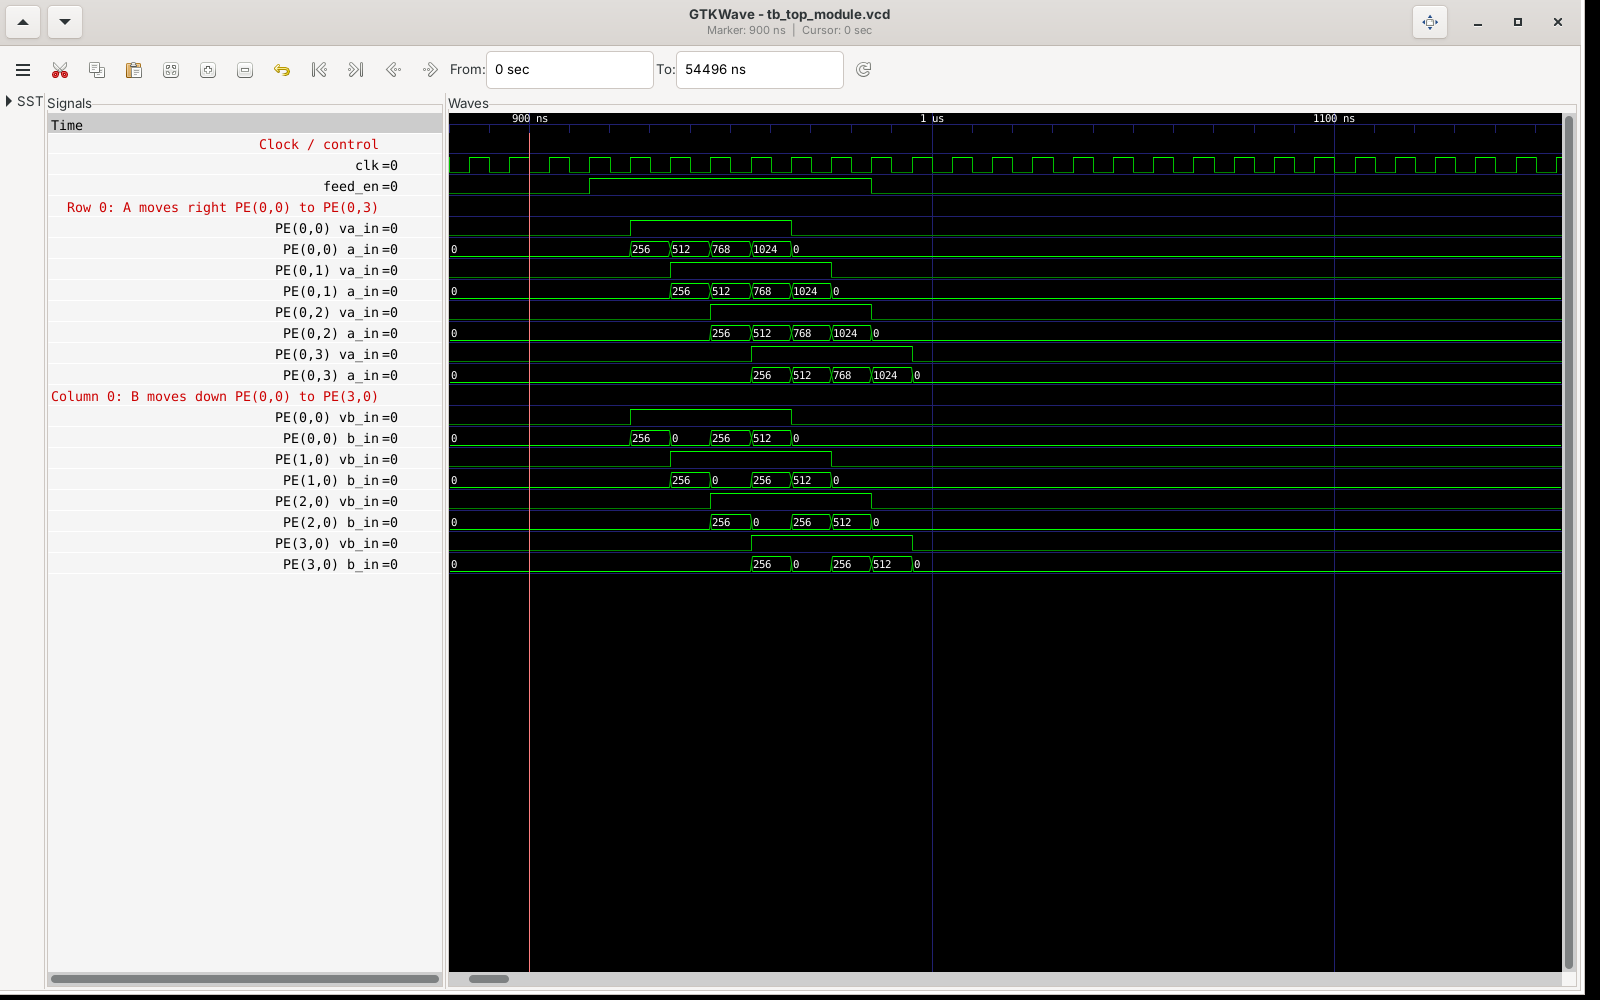
\includegraphics[width=0.80\textwidth]{04_pe_dataflow.png}\\[2pt]
{\footnotesize (b) Systolic data movement: row 0 of A passes PE(0,0)$\rightarrow$PE(0,3); column 0 of B passes PE(0,0)$\rightarrow$PE(3,0), one hop per clock.}
\caption{GTKWave captures of Test Case 2 from \texttt{tb\_top\_module.vcd}. Values are raw integers (inputs: 256 = 1.0; accumulators: 65536 = 1.0).}
\label{fig:wave}
\end{figure*}
\begin{figure*}[!t]
\centering
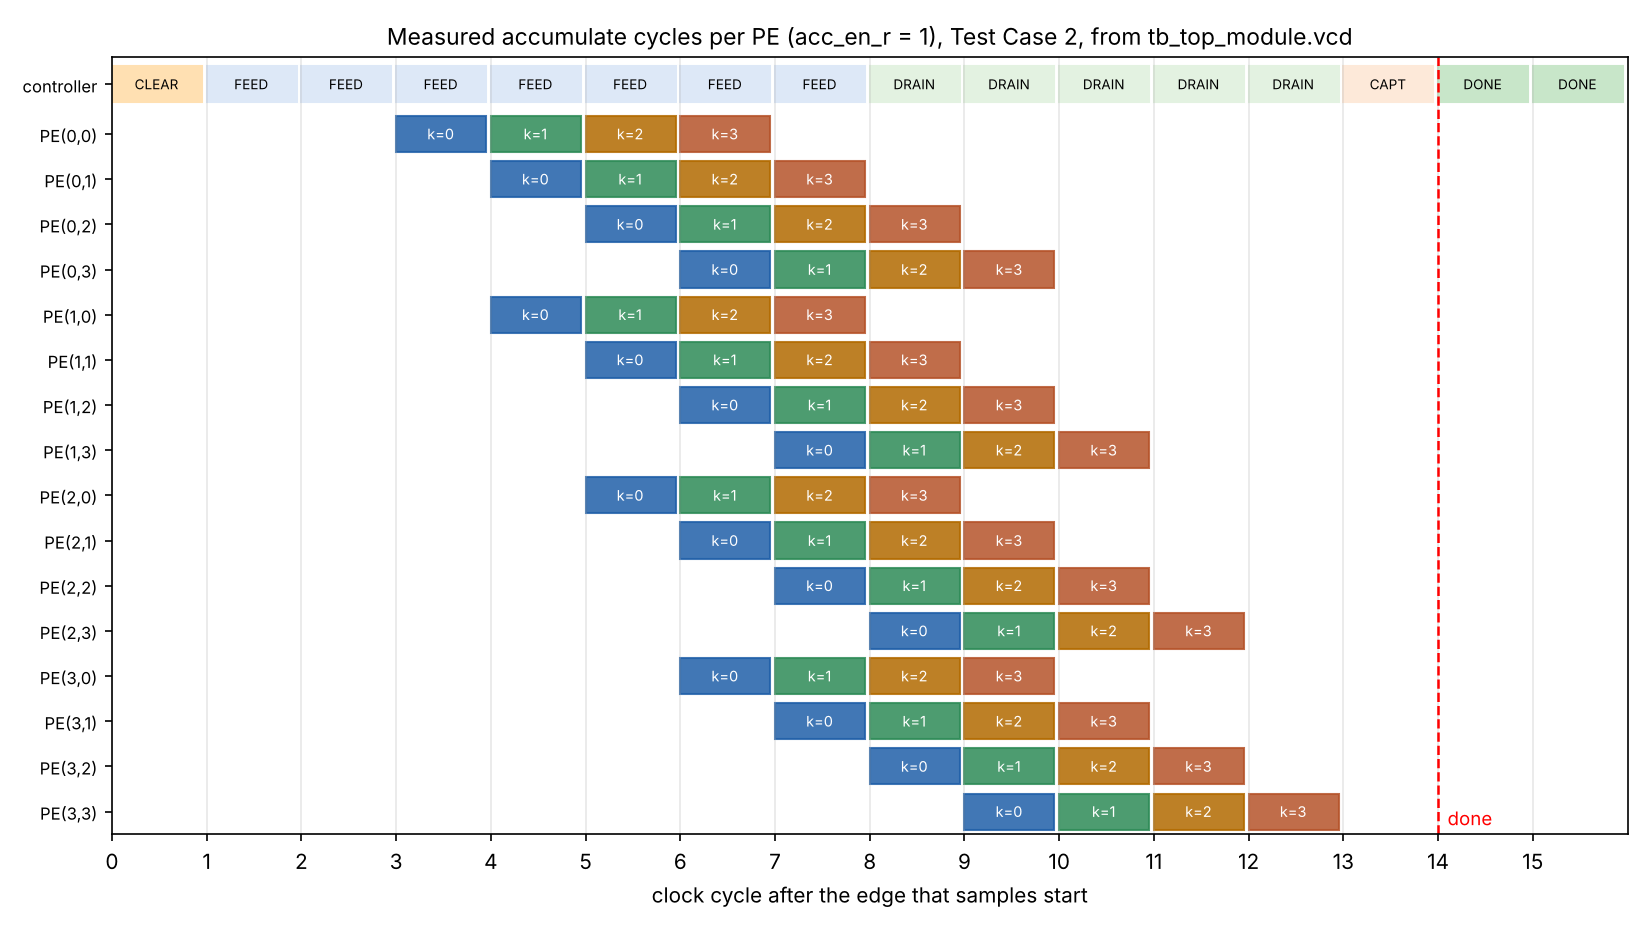
\includegraphics[width=0.82\textwidth]{execution_timing_from_vcd.png}
\caption{Accumulate cycles of every PE during Test Case 2, extracted from the simulation VCD.}
\label{fig:timing}
\end{figure*}
\section{Simulation Methodology}
Simulation used Icarus Verilog 12.0 with \texttt{-g2005 -Wall}, and all testbenches compile with zero warnings. Waveforms were dumped to VCD and inspected in GTKWave 3.3. All four testbenches are self-checking. Each computes the expected values itself with 64-bit integer arithmetic and compares them with the hardware outputs; none prints PASS without a comparison.
\begin{itemize}
\item \texttt{tb\_processing\_element}: a cycle-accurate reference model of the accumulator, pipeline register and forwarding registers. It covers signed MACs, valid gating, stall, clear, extreme operands, 40 random cycles and reset (109 checks).
\item \texttt{tb\_systolic\_array}: the testbench generates the skew itself, which tests the PE interconnect without the buffers or controller. It covers identity, constant, both signed extremes and 50 random cases (54 cases).
\item \texttt{tb\_top\_module}: full system through the host port. It checks all 16 elements of both \texttt{rd\_raw} and \texttt{rd\_q88}, plus \texttt{rd\_ovf}, and measures latency and sustained throughput (108 cases).
\item \texttt{tb\_sequential\_matmul}: verifies the baseline and measures its latency (20 cases).
\end{itemize}
The hardware results for the three required cases were also cross-checked against an independent NumPy model (\texttt{docs/reference\_model.py}). To test the testbench itself, four faults were injected into copies of the RTL (mutation testing).

\section{Results and Discussion}
\subsection{Functional results}
Table~\ref{tab:tests} summarizes the system-level cases, all of which pass. Test Case 1 multiplies by the identity matrix, and the output equals $A$. Test Case 2 uses
\[
A=\begin{bmatrix}1&2&3&4\\5&6&7&8\\9&1&2&3\\4&5&6&7\end{bmatrix},\ 
B=\begin{bmatrix}1&2&0&1\\0&1&2&0\\1&0&1&2\\2&1&0&1\end{bmatrix},
\]
for which both the hardware and the reference give
\[
C=\begin{bmatrix}12&8&7&11\\28&24&19&27\\17&22&4&16\\24&20&16&23\end{bmatrix}.
\]
Test Case 3 mixes negative and fractional operands, from $\pm1/256$ to $9.0$, and matches the reference exactly at full precision. For example, $C_{31} = -63.996094$ and $C_{02} = -14.101562$. In Test Case 4 every product is $(-128)^2$: the 34-bit accumulator holds the exact sum $2^{32}/2^{16} = 65536$, and the Q8.8 output saturates to $+127.996$ with \texttt{rd\_ovf}=1, as designed.

\begin{table}[t]
\caption{System-Level Verification (\texttt{tb\_top\_module})}
\label{tab:tests}
\centering\footnotesize
\begin{tabular}{@{}lr@{}}
\toprule
Test & Result \\ \midrule
TC1: $A \times I = A$ & 16/16 pass \\
TC2: general integer matrices & 16/16 pass \\
TC3: negative and fractional Q8.8 & 16/16 pass \\
TC4: extremes $(-128.0)\times(-128.0)$, saturation & 16/16 pass \\
TC5: zero matrix & 16/16 pass \\
TC6: back-to-back start (accumulator clear) & 16/16 pass \\
TC7: writes ignored while busy & 16/16 pass \\
100 random full-range matrices & 100/100 pass \\
Sustained-throughput run & 16/16 pass \\ \midrule
\textbf{Total} & \textbf{108/108 cases} \\ \bottomrule
\end{tabular}
\end{table}

Mutation testing gave the following results. A controller that drains one cycle short failed 107 of 108 cases, feeding $B$ row-wise failed 105, and removing sign extension in the MAC failed 104. The fourth mutant, which ignores the B-valid bit, passed. This is expected: in this design the two valid bits are always equal at every PE, so the mutant is functionally equivalent to the original.

\subsection{Waveforms}
Fig.~\ref{fig:wave}(a) shows Test Case 2 in GTKWave. The controller passes through CLEAR, FEED (steps 0--6), DRAIN and CAPTURE. The input lanes form the expected staircase, and \texttt{done} rises after 14 cycles. The accumulators settle at, for example, PE(0,0) $= 786432/65536 = 12$. Fig.~\ref{fig:wave}(b) follows row~0 of $A$ moving right and column~0 of $B$ moving down, one PE per clock.



\subsection{Measured timing}
Fig.~\ref{fig:timing} was produced by a script that reads the VCD and records, for each PE, the cycles in which its accumulate enable is high. PE$(i,j)$ accumulates in cycles $3+i+j$ to $6+i+j$, a diagonal wavefront that agrees with (\ref{eq:arr}) plus the constant pipeline offset. The last MAC occurs in cycle 12, capture in cycle 13, and \texttt{done} in cycle 14, which matches (\ref{eq:lat}).


\section{Performance Analysis}
\label{sec:perf}
\subsection{Cycle counts}
Table~\ref{tab:cyc} compares the two designs. Cycle counts were measured in simulation (latency: edges from the edge that samples \texttt{start} to \texttt{done}; period: \texttt{start} held high over four jobs). The systolic array needs 4.6$\times$ fewer cycles of latency and 4.3$\times$ fewer cycles per product.

PE utilization is $64 / (16 \times 15) = 26.7\%$. Each PE does its four MACs in a four-cycle window and is otherwise idle while the array fills, drains, clears and captures.

\begin{table}[t]
\caption{Cycle-Level Comparison (Simulation)}
\label{tab:cyc}
\centering\footnotesize
\begin{tabular}{@{}lrr@{}}
\toprule
Metric & Systolic & Sequential \\ \midrule
Latency (cycles) & 14 & 64 \\
Sustained period (cycles/product) & 15 & 65 \\
MACs per product & 64 & 64 \\
Peak parallel MACs & 16 & 1 \\
PE utilization & 26.7\% & 98.5\% \\ \bottomrule
\end{tabular}
\end{table}

\subsection{FPGA implementation}
Both designs were synthesized with Yosys \cite{yosys} and placed and routed with nextpnr \cite{shah2019} on a Lattice ECP5 LFE5U-25F \cite{ecp5ds} with a 100\,MHz constraint. The I/O pins were left unconstrained because no specific board was targeted. Placement is randomized, so three seeds were run. Table~\ref{tab:fpga} gives the post-route results.

\begin{table}[t]
\caption{Lattice ECP5-25F Post-Route Results}
\label{tab:fpga}
\centering\footnotesize
\begin{tabular}{@{}lrr@{}}
\toprule
Resource / metric & Systolic & Sequential \\ \midrule
LUT4 (of 24\,288) & 1\,787 & 193 \\
Flip-flops (of 24\,288) & 2\,150 & 42 \\
MULT18X18D (of 28) & 16 & 1 \\
Distributed-RAM write ports & 32 & 17 \\
Fmax, seeds 1/2/3 (MHz) & 102.0/122.0/127.8 & 82.2/84.4/83.2 \\
Fmax, median (MHz) & 122.0 & 83.2 \\ \midrule
Latency (ns, median Fmax) & \textbf{114.7} & 769.3 \\
Throughput (M products/s) & \textbf{8.14} & 1.28 \\ \bottomrule
\end{tabular}
\end{table}

At the median clock, the accelerator is 6.7$\times$ faster in latency and 6.4$\times$ faster in throughput (5.7$\times$ in latency at the worst seed for each design). This costs 16$\times$ the multipliers, 9.3$\times$ the LUTs and 51$\times$ the flip-flops. Most of the extra flip-flops are inter-PE forwarding registers, product registers and the 544-bit output register. A Yosys technology mapping to Xilinx 7-series (pre-route only, not a Vivado result) uses 16 DSP48E1 slices \cite{ug479}, 838 flip-flops and 384 LUTs. It needs fewer flip-flops because accumulators are absorbed into DSP registers.

\subsection{Design-space decisions}
Two optimizations were measured and kept. First, indexing the result bus as \texttt{result[rd\_addr*W +: W]} made Yosys build a variable multiplier and a 544-bit shifter. Rewriting it with constant part-selects reduced the 7-series mapping from 2\,495 to 1\,455 cells (17 to 16 DSPs). Second, the one-stage MAC reached only 97.2/95.7/91.0\,MHz across the three seeds (13-cycle latency, 135.8\,ns at the median). Adding the product register raised this to the values in Table~\ref{tab:fpga} at a cost of one cycle (114.7\,ns). Seed~1 alone would have favoured the one-stage design slightly (133.8 vs 137.2\,ns), which shows why a single place-and-route run is not a reliable basis for such decisions.

\section{Individual Contributions}
This project was carried out by a single student. Yash Dhankhar specified the architecture and fixed-point format and performed the RTL implementation of all modules and the baseline. The same student did the verification (testbenches, reference model and mutation tests), simulation and waveform analysis, synthesis and place-and-route experiments, diagrams, and this report.

\emph{Note for evaluators:} the course brief expects five group members, with each member's contributions shown in the report, video and repository history. That requirement cannot be met by a single-member team; no other contributors are listed, and the team-size requirement is to be confirmed with the instructor.

\section{Conclusion}
A 4$\times$4 output-stationary systolic array for signed Q8.8 matrix multiplication was designed in Verilog, verified with self-checking testbenches against independent references, and implemented on an ECP5 FPGA. It completes a product in 14 cycles (114.7\,ns at the median 122.0\,MHz post-route clock), against 64 cycles (769.3\,ns) for a sequential single-MAC design. That is a 6.7$\times$ reduction in latency obtained by trading area for parallelism. The measured per-PE timing confirms the systolic wavefront predicted by (\ref{eq:arr}).

\section{Future Scope}
\begin{itemize}
\item Overlap consecutive jobs with double-buffered accumulators to raise utilization towards the $2N-1$-cycle steady state.
\item Replace the 16-bit host port, whose 32 load cycles exceed the compute time, with wider or AXI-Stream inputs.
\item Tile larger matrices over the array and compare with weight-stationary dataflow \cite{jouppi2017,sze2017}.
\item Add INT8 and bfloat16 modes for neural-network inference.
\item Demonstrate the design on a physical FPGA board with a UART host link.
\end{itemize}

\begin{thebibliography}{00}
\bibitem{kung1979} H. T. Kung and C. E. Leiserson, ``Systolic arrays (for VLSI),'' in \emph{Sparse Matrix Proceedings 1978}, I. S. Duff and G. W. Stewart, Eds. Philadelphia, PA, USA: SIAM, 1979, pp. 256--282.
\bibitem{kung1982} H. T. Kung, ``Why systolic architectures?'' \emph{Computer}, vol. 15, no. 1, pp. 37--46, Jan. 1982.
\bibitem{kung1985} S. Y. Kung, ``VLSI array processors,'' \emph{IEEE ASSP Mag.}, vol. 2, no. 3, pp. 4--22, Jul. 1985.
\bibitem{jouppi2017} N. P. Jouppi \emph{et al.}, ``In-datacenter performance analysis of a tensor processing unit,'' in \emph{Proc. 44th Annu. Int. Symp. Comput. Archit. (ISCA)}, Toronto, ON, Canada, 2017, pp. 1--12.
\bibitem{chen2017} Y.-H. Chen, T. Krishna, J. S. Emer, and V. Sze, ``Eyeriss: An energy-efficient reconfigurable accelerator for deep convolutional neural networks,'' \emph{IEEE J. Solid-State Circuits}, vol. 52, no. 1, pp. 127--138, Jan. 2017.
\bibitem{sze2017} V. Sze, Y.-H. Chen, T.-J. Yang, and J. S. Emer, ``Efficient processing of deep neural networks: A tutorial and survey,'' \emph{Proc. IEEE}, vol. 105, no. 12, pp. 2295--2329, Dec. 2017.
\bibitem{genc2021} H. Genc \emph{et al.}, ``Gemmini: Enabling systematic deep-learning architecture evaluation via full-stack integration,'' in \emph{Proc. 58th ACM/IEEE Design Autom. Conf. (DAC)}, 2021, pp. 769--774.
\bibitem{samajdar2018} A. Samajdar, Y. Zhu, P. Whatmough, M. Mattina, and T. Krishna, ``SCALE-Sim: Systolic CNN accelerator simulator,'' arXiv:1811.02883, 2018.
\bibitem{ieee1364} \emph{IEEE Standard for Verilog Hardware Description Language}, IEEE Std 1364-2005, 2006.
\bibitem{yosys} C. Wolf, ``Yosys Open SYnthesis Suite.'' [Online]. Available: \url{https://yosyshq.net/yosys/}
\bibitem{shah2019} D. Shah \emph{et al.}, ``Yosys+nextpnr: An open source framework from Verilog to bitstream for commercial FPGAs,'' in \emph{Proc. IEEE 27th Annu. Int. Symp. Field-Programmable Custom Comput. Mach. (FCCM)}, 2019, pp. 1--4.
\bibitem{ecp5ds} Lattice Semiconductor, \emph{ECP5 and ECP5-5G Family Data Sheet}, FPGA-DS-02012.
\bibitem{ug479} Xilinx, \emph{7 Series DSP48E1 Slice User Guide}, UG479.
\end{thebibliography}

\end{document}
